[200~v\textsuperscript{o}] proinde non fuisse opus follium multiplicatione. Utroque modo \edtext{res exitum}{\lemma{res}\Afootnote{ \textit{ (1) }\ est ex \textit{ (2) }\ exitum \textit{ L}}} infallibiliter nanciscitur. Sed si haec omnia ponantur irrita, superest tamen quod decipere non potest. Pone enim pondere contrario ad deprimendum opus esse, pone non plus aeris attrahere posse lignum in follem, quam quantum in ipso est ac proinde levitatem fore parvam minoremque quam est ponderis deprimentis gravitas\protect\index{Sachverzeichnis}{gravitas}, necesse est tamen vinci pondus deprimens applicatis viribus mechanicis\protect\index{Sachverzeichnis}{vis!mechanica}, ut statera\protect\index{Sachverzeichnis}{statera} aut trochlea\protect\index{Sachverzeichnis}{trochlea}. Si Trochleam\protect\index{Sachverzeichnis}{trochlea} adhibeas poterit recta ascendere descendereque follis, et tamen elevare pondus. Si contrapondio careri potest longe mirabilior erit illa rectilinea ascensio et descensio, cujus causam nemo videt; nec nisi subtilissimo ratiocinio deprehendet, etsi omnia perviderit. Si hic casus sit possibilis ut aqua ipsa seu aer resistat attractioni ultra quam est ligni capacitas, adhibenturque folles multiplicati nihil necesse est multiplicari tubos, modo ex pleno jam folle regressus in tubulum si impeditus, valvula quadam se claudente etc.\pend 
   \begin{center}                   
   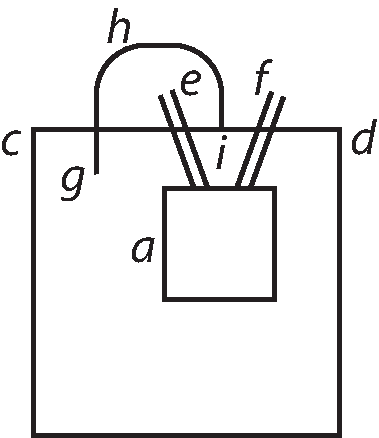
\includegraphics[width=0.3\textwidth]{images/38_200v}
   \\ \textit{[Fig. 1]} \\
   \end{center}
\pstart Nota pro valvis\protect\index{Sachverzeichnis}{valvae} et obicibus adhiberi \edtext{possent}{\lemma{adhiberi}\Afootnote{ \textit{ (1) }\ possunt \textit{ (2) }\ possent \textit{ L}}} duo plana levigata sibi exacte imposita quae a se separantur inclinatione, aliter non maxima vi. Nota posset etiam loco valvularum\protect\index{Sachverzeichnis}{valvae} separatarum ita agi ut quilibet follis tubum habeat diversum, quilibet autem tubus exeat in aeris, regionem cum altero inconnexam, ut si aqua intercedente dividatur. Esto follis \textit{a} aquae superficies \textit{cd}. Tubi duo \textit{e}, \textit{f} separator \textit{ghi}. Sed non puto aliquod profuturum. Quia liquido aliquo connectuntur. Sed si non nisi duro, ut si claudantur valvis\protect\index{Sachverzeichnis}{valvae} pressioni resistet corporis durities, nec ab altero in alterum derivabitur. Nihil ergo restat, quod putem propositioni objici posse, nisi valvas\protect\index{Sachverzeichnis}{valvae} non adeo exacte clausum iri. Sed puto ego clausuram etiam leve sufficere. Et praeterea ut fiat exacta effici potest, si distrahatur intus paulum aer primi follis continuata assurrectione, ita enim ipse spatio angustato seu contracto rimas claudet. Et si intus obices sint duplicati. Aut si aliqua in obice vis elastica\protect\index{Sachverzeichnis}{vis!elastica}, qua ipse se \edtext{ad rimas exacte claudendas expendat}{\lemma{se}\Afootnote{ \textit{ (1) }\ cogat \textit{ (2) }\ ad rimas exacte claudendas expendat \textit{ L}}}. Aut si tantum circumgyretur aliquid et infra hoc rursus aliquid etc. et sic quoties lubet, et non possunt aperiri valvae\protect\index{Sachverzeichnis}{valvae} toties multiplicatae nisi his omnibus ita sibi superimpositis, ut correspondeant foramina. Et possunt haec duplicaturae sibi superpositae exacte levigatae esse ut distrahi a se non possint sed super se converti possint ita nihil aeris per transibit, ut patet. Sed danda simul opera est ne nimio tempore ad redaperiendum opus sit quod facile fieri potest ut exigua \edtext{immutatione}{\lemma{exigua}\Afootnote{ \textit{ (1) }\ permutatione \textit{ (2) }\ immutatione \textit{ L}}} \edtext{redeat}{\lemma{}\Afootnote{immutatione \textbar\ facile \textit{ gestr.}\ \textbar\ redeat \textit{ L}}} foramen subito. Si recta ascendat \edtext{follis}{\lemma{ascendat}\Afootnote{ \textit{ (1) }\ leve \textit{ (2) }\ follis \textit{ L}}}. Non opus erit vectis\protect\index{Sachverzeichnis}{vectis} cujus crassities non nihil obstat. Etsi esset instar aciei cultri. \pend 